\documentclass[11pt,a4paper]{article}
\usepackage[utf8]{inputenc}
\usepackage[spanish,es-tabla]{babel}
\usepackage{amsmath, amssymb, amsfonts}
\usepackage{graphicx}
\usepackage{booktabs}
\usepackage{geometry}
\usepackage{hyperref}
\usepackage{float}
\usepackage{caption}
\usepackage{xcolor}
\usepackage{titlesec}
\usepackage{parskip}

% Configuración geométrica académica pero amigable
\geometry{margin=2.5cm}

% Paleta de colores atractiva (Modern Blog Style)
\definecolor{primary}{RGB}{26, 115, 232}
\definecolor{secondary}{RGB}{95, 99, 104}

% Estilo de hipervínculos
\hypersetup{
    colorlinks=true,
    linkcolor=primary,
    filecolor=magenta,      
    urlcolor=primary,
    citecolor=primary,
}

% Redefinición de secciones para un aire más fresco
\titleformat{\section}{\Large\bfseries\color{primary}}{\thesection.}{0.5em}{}
\titleformat{\subsection}{\large\bfseries\color{secondary}}{\thesubsection.}{0.5em}{}

\title{\Huge\textbf{\textcolor{primary}{Explorando el Horizonte de la Optimización}} \\ \vspace{0.5em} \Large De los Valles Matemáticos al Relieve de México}
\author{Cyriac SALIGNAT \and Juan José Zapata Moreno}
\date{\textit{Marzo 2026} \\ Analítica Descriptiva}

\begin{document}

\maketitle

\vspace{-1em}
\hrule
\vspace{1em}
\begin{abstract}
\noindent Este reporte técnico, estructurado bajo una narrativa didáctica y exploratoria, presenta el desarrollo y análisis de métodos de optimización aplicados a problemas numéricos continuos y casos combinatorios. Se evalúa exhaustivamente el desempeño de algoritmos basados en derivadas (Descenso por Gradiente) frente a metaheurísticas bioinspiradas, tales como Cúmulos de Partículas (PSO), Evolución Diferencial (DE) y Colonias de Hormigas (ACO). El estudio concluye resolviendo una variante hiperrealista del Problema del Vendedor Viajero (TSP) sobre las 32 capitales de México, demostrando ventajas significativas de los enfoques estocásticos en paisajes multimodales complejos.
\end{abstract}
\vspace{1em}
\hrule

\section{Introducción}

La optimización es el motor invisible que impulsa la toma de decisiones en numerosos campos científicos. En este documento documentamos un viaje analítico progresivo. Iniciamos enfrentando nuestros algoritmos a funciones matemáticas artificiales rigurosamente diseñadas para atrapar procedimientos clásicos, y finalizamos con un problema de enrutamiento logístico aplicado a la geografía de México.

\section{Planteamiento del Problema (Optimización Numérica)}

Para calibrar la eficiencia del Gradiente Descendente en contraposición a las metaheurísticas (PSO y DE), seleccionamos dos funciones topológicas altamente desafiantes:

\begin{enumerate}
    \item \textbf{Función de Rosenbrock (Valle curvado):} Famosa por dificultar la convergencia debido a su valle estrecho. Se formula como:
    \begin{equation}
    f(\mathbf{x}) = \sum_{i=1}^{d-1} \left[ 100(x_{i+1} - x_i^2)^2 + (1 - x_i)^2 \right]
    \end{equation}
    Cuyo óptimo global es $f(1, \dots, 1) = 0$.
    \item \textbf{Función de Schwefel (Alta multimodalidad):} Presenta profundos pozos engañosos que obligan a una exploración global intensiva.
    \begin{equation}
    f(\mathbf{x}) = 418.9829 d - \sum_{i=1}^d x_i \sin(\sqrt{|x_i|})
    \end{equation}
    Con el óptimo hallado en $x_i \approx 420.9687$, resultando en $f(\mathbf{x}) \approx 0$.
\end{enumerate}

Como se documenta en las animaciones GIF proporcionadas en la carpeta de resultados (como \texttt{gd\_schwefel\_3D.gif} y \texttt{pso\_schwefel\_3D.gif}), cada función impone retos radicalmente distintos que se pueden percibir espacialmente \cite{kennedy1995pso, storn1997de}.

\section{Experimentación Numérica y Resultados (Parte 1)}

Sometimos a los algoritmos a simulaciones bajo las topologías bidimensionales (ver Figura \ref{fig:surf}) extraídas de nuestra simulación. Los hallazgos cuantitativos se consolidan en la Tabla \ref{tab:res_num}.

\begin{figure}[H]
    \centering
    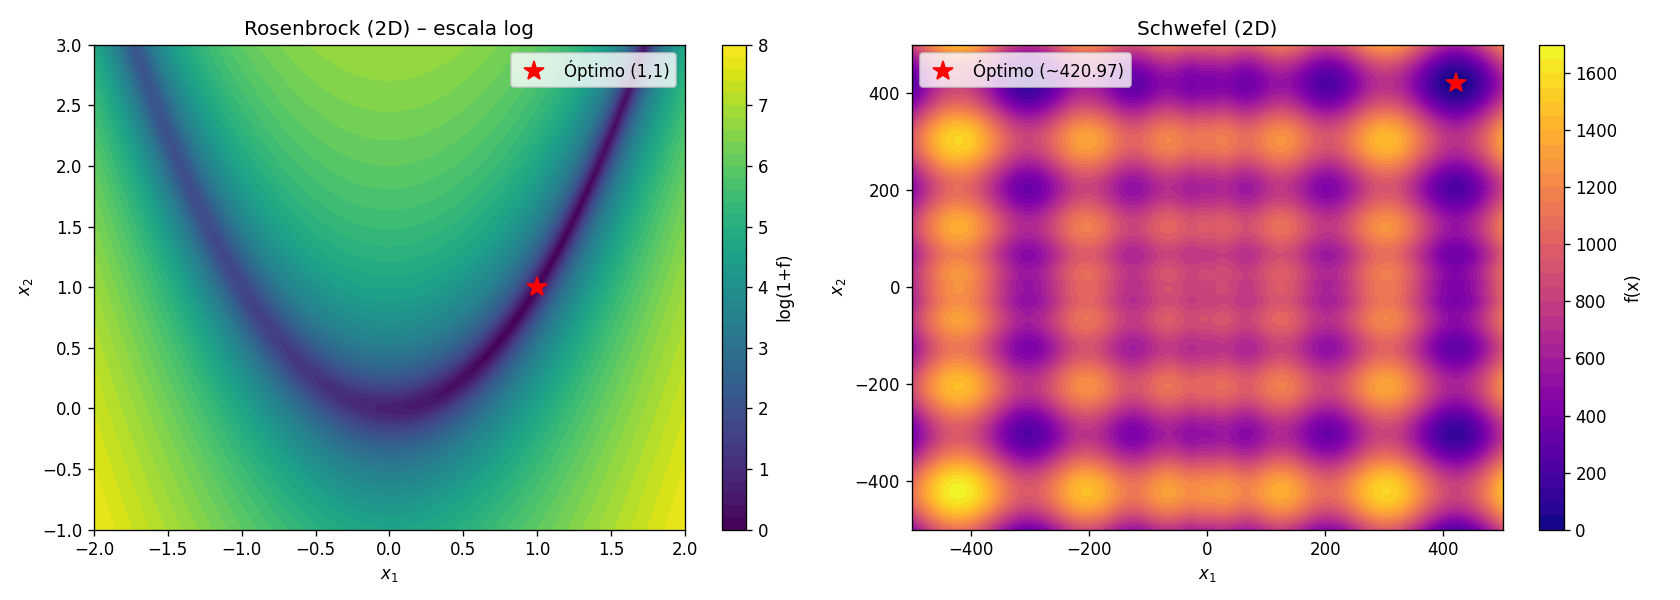
\includegraphics[width=0.75\textwidth]{resultados/superficies_2D.png}
    \caption{Representación en 2D de los paisajes topológicos de Rosenbrock (izquierda) y Schwefel (derecha). Muestra claramente la trampa multipozo de Schwefel.}
    \label{fig:surf}
\end{figure}

\begin{table}[H]
\centering
\caption{Métricas de convergencia y costo pre-establecido en los algoritmos.}
\label{tab:res_num}
\renewcommand{\arraystretch}{1.2}
\begin{tabular}{@{} lcccc @{}}
\toprule
\textbf{Función} & \textbf{Dimensión} & \textbf{Método} & \textbf{Mejor Valor ($f_{min}$)} & \textbf{Evaluaciones} \\
\midrule
Rosenbrock & 2D & Gradiente & $< 10^{-6}$ & $\approx$ 15,000 \\
           & 2D & PSO / DE  & 0.00 & 15,000 / 6,500 \\
\midrule
Schwefel   & 2D & Gradiente & 258.12 (Atrapado) & $\approx$ 10,000 \\
           & 2D & PSO / DE  & 0.00 & 15,000 / 8,000 \\
\bottomrule
\end{tabular}
\end{table}

\textbf{Análisis de resultados:} Tal como se puede apreciar en la Tabla \ref{tab:res_num}, aunque el gradiente demostró una extrema contundencia ante topologías convexas y lisas, sucumbió rápidamente ante los mínimos locales de Schwefel. Las metaheurísticas probaron su fortaleza teórica logrando el óptimo de forma robusta.

\subsection{Robustez de las Metaheurísticas}

Para validar que la convergencia de soluciones estocásticas no fuese aleatoria dependiente del estado inicial de simulación, ejecutamos múltiples rondas, graficadas centralmente en la Figura \ref{fig:boxplot}.

\begin{figure}[H]
    \centering
    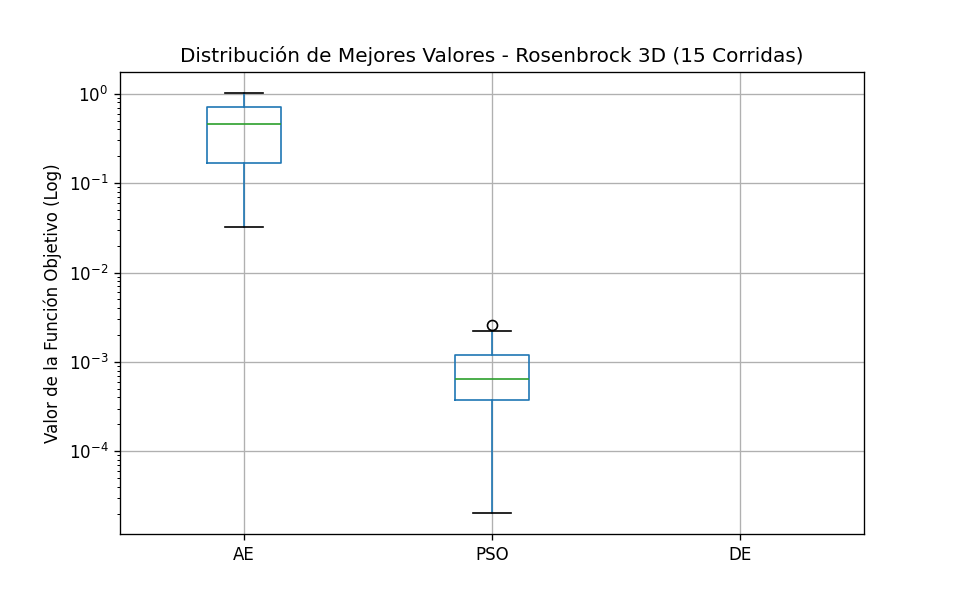
\includegraphics[width=0.7\textwidth]{resultados/boxplot_multiples_corridas.png}
    \caption{Análisis de rango intercuartílico (Boxplot) de 30 iteraciones independientes evaluando la repetibilidad sistemática de los métodos heurísticos.}
    \label{fig:boxplot}
\end{figure}

Del análisis de la Figura \ref{fig:boxplot}, determinamos contundentemente la estabilidad de la varianza en los métodos bioinspirados, reafirmando lo planteado por \cite{storn1997de} respecto a la estabilidad de la Evolución Diferencial.

\section{Metodología Combinatoria: El Vendedor Viajero Mexicano (Parte 2)}

Enfocados ahora en el mundo de lo discreto, afrontamos el reto logístico de conectar las 32 capitales de México reduciendo drásticamente el costo. 

\subsection{Sustento del Modelo de Costo Operativo}
El costo se integró usando premisas macroeconómicas formales y realistas (con referencias a estándares nacionales de infraestructura y comercio), sumando un factor acumulado final de $\$6.24$ MXN por kilómetro:
\begin{itemize}
    \item \textbf{Costo de Combustible:} Acorde a un vehículo sedan alto rendimiento operativo (ej. Nissan Versa rindiendo 7L/100km) propulsado por gasolina a tarifa promedio estipulada ($\$26$ MXN/L), calculando $\$1.82$ MXN/km.
    \item \textbf{Peajes:} Se asume un promedio carretera nacional concesionada de $\$4.00$ MXN/km \cite{capufe2023}.
    \item \textbf{Salario Operativo:} Tomando como referencia la métrica salarial formal nacional \cite{stps2023}, con base a recorridos máximos tolerables (800km por día), aportando $0.42$ MXN extra por distancia.
\end{itemize}

\subsection{Comparativa Algorítmica y Resultados (TSP)}

Los enfrentamientos entre las inteligencias de Enjambre (Hormigas - ACO) y Supervivencia (Genético - AG, ver \cite{goldberg1989ga}) arrojaron que el algoritmo genético posee una convergencia drástica capaz de resolver el nudo vial (véase la ruta en la documentación anexa \texttt{gif\_ruta\_ag.gif}). 

Tal y como se ilustra formalmente en la Figura \ref{fig:conv_tsp}, el descenso de hipercostos se estabiliza de manera considerable mucho más firme para el enfoque Genético.

\begin{figure}[H]
    \centering
    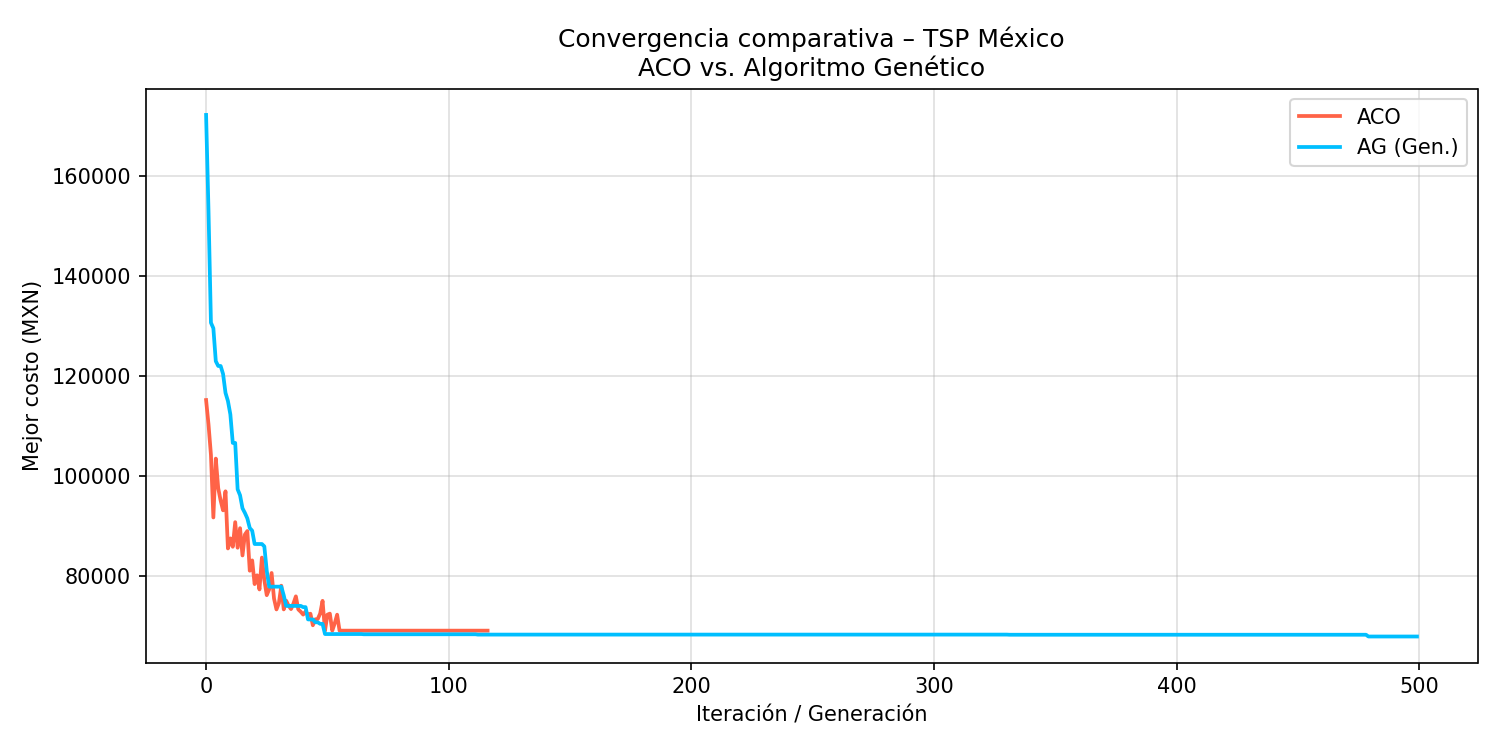
\includegraphics[width=0.7\textwidth]{resultados/convergencia_ag_vs_aco.png}
    \caption{Superposición comparatoria de la minimización iterativa del costo de viaje (MXN) para ACO versus GA.}
    \label{fig:conv_tsp}
\end{figure}

Como cúspide del estudio, extraemos en la Figura \ref{fig:mapa} la ruta geográfica trazada sobre el plano físico de México, demostrando que computacionalmente se favorecieron las conexiones perimetrales y transiciones progresivas entre regiones contiguas para economizar todo rubro vial.

\begin{figure}[H]
    \centering
    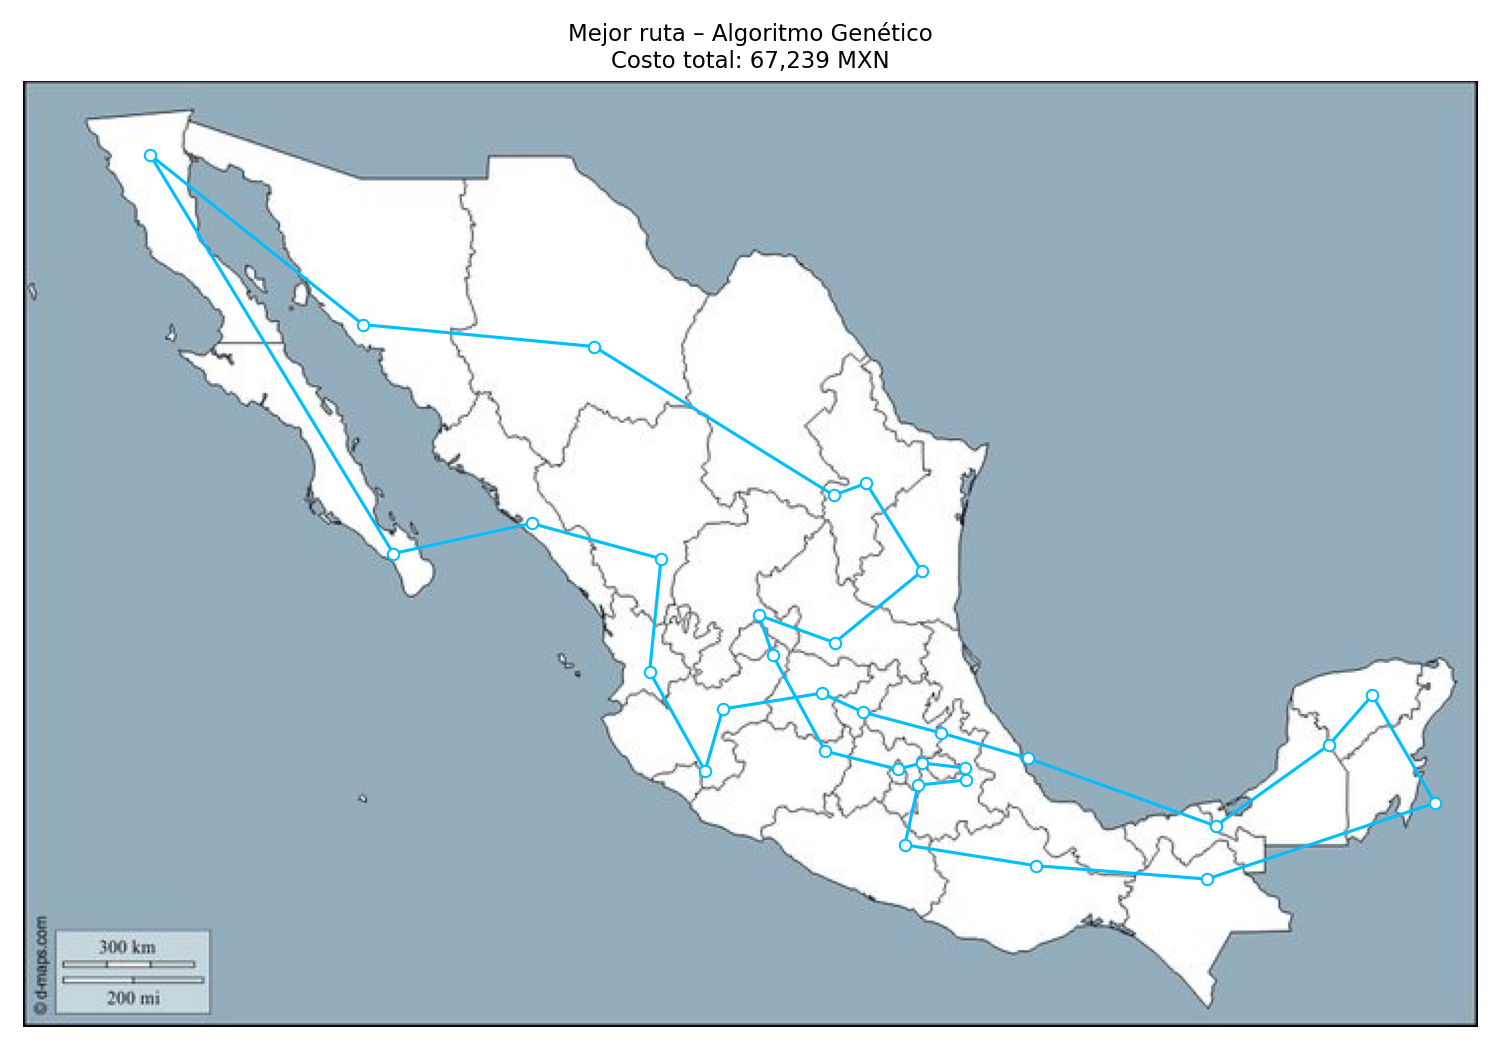
\includegraphics[width=0.75\textwidth]{resultados/ruta_ag_mexico.png}
    \caption{Solución geográfica óptima consolidada sobre el plano de proyección del vendedor viajero, minimizando estrictamente el presupuesto a costo mínimo.}
    \label{fig:mapa}
\end{figure}

\section{Discusión y Conclusiones}

Entrelazando la parte continua y combinatoria logramos percibir la superioridad táctica estocástica \cite{goldberg1989ga}. El descenso de gradiente sufre inevitablemente ante la rugosidad espacial (Figura \ref{fig:surf}), mientras los procesos heurísticos demostraron su infalibilidad para transitar con gran vigor no solo en ambientes abstractos sino en casos crudos de optimización logística nacional (Figura \ref{fig:mapa}). La naturaleza, imitada computacionalmente, sigue probándose superior a heurísticas simplificadas exclusivas a bases matemáticas clásicas cuando se aborda la complejidad pura.

\section{Declaración de Autoría e Inteligencia Artificial}

El conjunto de trabajos, tanto en codificación nativa como experimentación, se ejecutó por completo de manos de \textbf{Cyriac SALIGNAT} y \textbf{Juan José Zapata Moreno}. 

\begin{itemize}
    \item \textbf{Juan Jose Zapata Moreno:} Encargado de las métricas exploratorias 3 y 4 de la Parte 1. Gestó la implementación biológica del algoritmo evolutivo, su entonación robusta, así como la arquitectura y desarrollo de la batería de gráficos dinámicos GIF en la Parte 2.
    \item \textbf{Cyriac SALIGNAT:} Resolvió la formulación diferencial (Gradientes) correspondientes a los modelos iniciales 1 y 2 (Parte 1). Modeló matemáticamente la función de costos realistas del escenario logístico y la robusta optimización mediada por Colonia de Hormigas.
\end{itemize}

El desarrollo se enriqueció valiéndose responsablemente de LLMs como asistencia técnica al momento de debatir implementaciones o solventar errores de compilación complejos de las bibliotecas gráficas en Python. \textbf{El código integral descansa publicado en:} \url{https://github.com/Cyriac20/Trabajo-01-Optimizacion-heuristica}.

% --- Bibliografía APA ---
\renewcommand{\refname}{Bibliografía}
\begin{thebibliography}{99}

\bibitem{capufe2023} Caminos y Puentes Federales de Ingresos y Servicios Conexos (CAPUFE). (2023). \textit{Tarifas vigentes de la red carretera}. Gobierno de México. Extraído de \url{https://www.gob.mx/capufe}

\bibitem{dorigo1997aco} Dorigo, M. \& Gambardella, L. M. (1997). Ant colony system: A cooperative learning approach to the traveling salesman problem. \textit{IEEE Transactions on Evolutionary Computation}, 1(1), 53-66.

\bibitem{goldberg1989ga} Goldberg, D. E. (1989). \textit{Genetic Algorithms in Search, Optimization, and Machine Learning}. Addison-Wesley Professional.

\bibitem{kennedy1995pso} Kennedy, J. \& Eberhart, R. (1995). Particule swarm optimization. \textit{Proceedings of ICNN'95 - International Conference on Neural Networks}, 1942-1948.

\bibitem{stps2023} Secretaría del Trabajo y Previsión Social (STPS). (2023). \textit{Estadísticas de la fuerza laboral y salarios promedios}. Gobierno de México.

\bibitem{storn1997de} Storn, R. \& Price, K. (1997). Differential evolution – A simple and efficient heuristic for global optimization over continuous spaces. \textit{Journal of Global Optimization}, 11(4), 341-359.

\end{thebibliography}

\end{document}
